\documentclass{standalone}
\usepackage{tikz}
\usepackage{ctex,siunitx,ninecolors}
\setCJKmainfont{Noto Serif CJK SC}
\usepackage{tkz-euclide}
\usepackage{amsmath}
\usetikzlibrary{patterns, calc}
\usetikzlibrary {decorations.pathmorphing, decorations.pathreplacing, decorations.shapes,3d}
\newcommand{\posthead}[2][gray]{
  \begin{scope}[#2]
    \fill[left color=#1,right color= #1,middle color=#1!20](0,0)ellipse(0.05 and 0.02);
    \fill[left color=#1,right color= #1,middle color=#1!20](0.05,0)rectangle(-0.05,0.07);
    \fill[left color=#1,right color= #1,middle color=#1!20](-0.06,0.07)arc(-180:0:0.06 and 0.02)--(0.06,0.15)--(0.05,0.16)--(-0.05,0.16)--(-0.06,0.15)--cycle;
    \fill[#1!50!gray](0,0.16)ellipse(0.05 and 0.02);
    \foreach \x in {75,45,15,-15,-45,-75}
    {
      \draw[very thin,#1!50!gray]({0.05*sin(\x)},{0.16-0.02*cos(\x)})--({0.06*sin(\x)},{0.15-0.02*cos(\x)})--++(0,-0.08);
    }
  \end{scope}
}
\newcommand\dlj[2][0]{
  \begin{scope}[#2,scale=1.8]
    \begin{scope}[z={(10:10mm)},x={(150:10mm)}]
      \begin{scope}[canvas is yz plane at x=-0.25]
        \draw[fill=lightgray](0,-0.5)rectangle(-0.1,0.5);
      \end{scope}
      \begin{scope}[canvas is xy plane at z=-0.5]
        \draw[fill=darkgray](0.25,-0.1)rectangle(-0.25,0);
      \end{scope}
      \begin{scope}[canvas is zx plane at y=0]
        \draw[fill=gray](-0.5,-0.25)rectangle(0.5,0.25);
      \end{scope}
      \begin{scope}[canvas is yz plane at x=-0.2]
        \draw[fill=lightgray!50](0,-0.4)rectangle(1.2,0.4);
        \foreach \x in {-30,-20,...,20}
        {
          \draw[ultra thin] ([shift=(\x:0.6)]0.4,0)--++(\x:-0.1);
          \draw[ultra thin] ([shift=(\x+5:0.6)]0.4,0)--++(\x+5:-0.08);
          \foreach \y in {1,2,3,4,6,7,8,9}
          {
            \draw[ultra thin] ([shift=(\x+\y:0.6)]0.4,0)--++(\x+\y:-0.05);
          }
        }
        \draw[ultra thin] ([shift=(30:0.6)]0.4,0)--++(30:-0.1);
        \draw[very thin,red] (0.4,0)--++(#1:0.65)(0.4,0)--++(#1:-0.05);
        \draw[fill=gray](0.4,0)circle(0.02);
        \draw[very thin,fill=darkgray](0.3,-0.1)--++(0.15,0)arc(-90:90:0.1)--(0.3,0.1)--(0.3,0.05)--++(0.15,0)arc(90:-90:0.05)--(0.3,-0.05)--cycle;
        \draw[fill=cyan!20,fill opacity=0.5,very thin](0.3,-0.35)rectangle(1.1,0.35);
        \coordinate (in) at (0.2,0.25);
        \coordinate (out) at (0.2,-0.25);
        \fill[darkgray](in)circle(0.8pt)(out)circle(0.8pt);
      \end{scope}
      \begin{scope}[canvas is xy plane at z=-0.4]
        \draw[fill=darkgray](0.2,1.2)rectangle(-0.2,0);
      \end{scope}
      \begin{scope}[canvas is yz plane at x=-0.25]
        \draw[fill=lightgray!50](1.3,-0.45)rectangle(1.2,0.45);
      \end{scope}
      \begin{scope}[canvas is xy plane at z=-0.45]
        \draw[fill=darkgray](0.25,1.2)rectangle(-0.25,1.3);
      \end{scope}
      \begin{scope}[canvas is zx plane at y=1.3]
        \draw[fill=gray](-0.45,-0.25)rectangle(0.45,0.25);
      \end{scope}
    \end{scope}
    \node at (in)[below]{\scalebox{0.5}{$+$}};
    \node at (out)[below]{\scalebox{0.5}{$-$}};
  \end{scope}
}
\begin{document}
\small
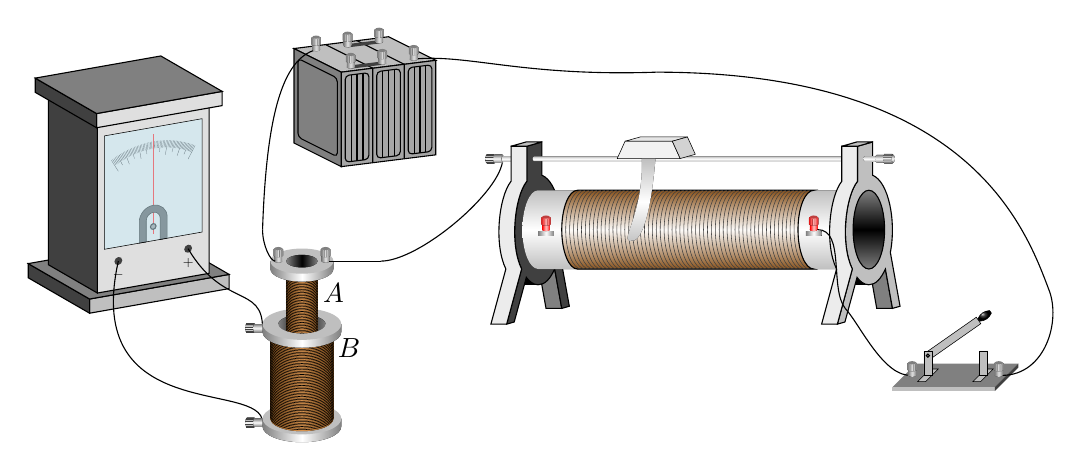
\begin{tikzpicture}[>=latex,scale=1]
  \draw(-1.95,0.9)..controls(-1.95,0.5)and(-3.0,-0.4)..(-3.5,-0.4);
  \fill[top color=gray,bottom color=gray,middle color=white](-2.15,0.9)ellipse(0.02 and 0.06);
  \fill[top color=gray,bottom color=gray,middle color=white](-2.15,0.84)rectangle(-2.05,0.96);
  \foreach \x in {75,45,15,-15,-45,-75}
  {
    \draw[very thin,darkgray]({-2.15-0.02*cos(\x)},{0.9+0.06*sin(\x)})--++(0.1,0);
  }
  % \node at (-2.1,0.9)[above]{$C$};
  \fill[gray](-2.05,0.9)ellipse(0.02 and 0.06);
  \fill[top color=gray,bottom color=gray,middle color=white](-2.05,0.9)ellipse(0.02 and 0.05);
  \fill[top color=gray,bottom color=gray,middle color=white](-2.05,0.85)rectangle(-1.95,0.95);
  \fill[gray](-1.95,0.9)ellipse(0.02 and 0.05);
  \fill[top color=lightgray,bottom color=lightgray,middle color=white](-1.95,0.9)ellipse(0.01 and 0.03);
  \fill[top color=lightgray,bottom color=lightgray,middle color=white](-1.95,0.87)rectangle(-1.6,0.93);
  \fill[gray,draw=black](-1.455,-0.692)--(-1.400,-1.000)--(-1.200,-1.000)--(-1.290,-0.500)--cycle;
  \fill[darkgray,draw=black](-1.644, 1.059)--(-1.644, 0.614)..controls(-1.797, 0.425)and(-1.866,-0.181)..(-1.710,-0.500)--(-1.900,-1.200)--(-1.804,-1.173)--(-1.650,-0.606)..controls(-1.619,-0.648)and(-1.568,-0.700)..(-1.500,-0.700)..controls(-1.411,-0.700)and(-1.345,-0.620)..(-1.290,-0.500)--(-1.200,-1.000)--(-1.104,-0.973)--(-1.227,-0.289)..controls(-1.150, 0.109)and(-1.249, 0.607)..(-1.452, 0.691)--(-1.452, 1.114)--cycle;
  \fill(-1.676,-0.700)--(-1.650,-0.606)..controls(-1.619,-0.648)and(-1.568,-0.700)..(-1.500,-0.700)--cycle;
  \fill[lightgray!30,draw=black](-1.844, 1.059)--(-1.844, 0.614)..controls(-1.997, 0.425)and(-2.066,-0.181)..(-1.910,-0.500)--(-2.100,-1.200)--(-1.900,-1.200)--(-1.710,-0.500)..controls(-1.866,-0.181)and(-1.797, 0.425)..(-1.644, 0.614)--(-1.644, 1.059)--cycle;
  \fill[lightgray,draw=black,line join=round](-1.844,1.059)--(-1.644,1.059)--(-1.452,1.114)--(-1.652,1.114)--cycle;
  \fill[top color=lightgray,bottom color=lightgray,middle color=white](-1.5,-0.5)arc(270:90:0.2 and 0.5)--(2.5,0.5)--(2.5,-0.5)--cycle;
  \fill[top color=brown4,bottom color=brown4,middle color=brown9!10,draw=black](-1,-0.5)arc(270:90:0.2 and 0.5)--(2,0.5)arc(90:270: 0.2 and 0.5)--cycle;
  \foreach \x in {-0.95,-0.9,...,1.98} { \draw[very thin,darkgray] (\x,-0.5)arc(270:90:0.2 and 0.5);}
  \fill[left color=gray,right color=gray,middle color=white](-1.5,-0.08)rectangle(-1.3,-0.02);
  \fill[left color=gray,right color=gray,middle color=white](1.9,-0.08)rectangle(2.1,-0.02);
  \fill[top color=lightgray,bottom color=lightgray,middle color=white](-1.55,0.87)arc(270:90:0.02 and 0.03)--(2.4,0.93)--(2.4,0.87)--cycle;
  \draw[fill=lightgray!20,very thin,line join=round](-0.396,1.123)--(-0.496,0.903)--( 0.304,0.903)--( 0.204,1.123)--cycle;
  \draw[fill=lightgray!40,very thin,line join=round](-0.396,1.123)--( 0.204,1.123)--( 0.396,1.177)--(-0.204,1.177)--cycle;
  \draw[fill=lightgray!70,very thin,line join=round]( 0.204,1.123)--( 0.396,1.177)--( 0.496,0.957)--( 0.304,0.903)--cycle;
  \fill[top color=lightgray,bottom color=lightgray,middle color=white](-0.182, 0.903)..controls(-0.163, 0.225)and(-0.446,-0.127)..(-0.341,-0.142)..controls(-0.181,-0.193)and(-0.066, 0.229)..(-0.010, 0.903);
  \fill(2.524,-0.700)--(2.700,-0.700)..controls(2.632,-0.700)and(2.581,-0.648)..(2.550,-0.606)--cycle;
  \fill[gray,draw=black](2.910,-0.500)--(3.000,-1.000)--(2.800,-1.000)--(2.745,-0.692)--cycle;
  \fill[lightgray,draw=black](2.556, 1.059)--(2.556, 0.614)..controls(2.403, 0.425)and(2.334,-0.181)..(2.490,-0.500)--(2.300,-1.200)--(2.396,-1.173)--(2.550,-0.606)..controls(2.581,-0.648)and(2.632,-0.700)..(2.700,-0.700)..controls(2.789,-0.700)and(2.855,-0.620)..(2.910,-0.500)--(3.000,-1.000)--(3.096,-0.973)--(2.973,-0.289)..controls(3.050, 0.109)and(2.951, 0.607)..(2.748, 0.691)--(2.748, 1.114)--cycle;
  \fill[lightgray!30,draw=black](2.356, 1.059)--(2.356, 0.614)..controls(2.203, 0.425)and(2.134,-0.181)..(2.290,-0.500)--(2.100,-1.200)--(2.300,-1.200)--(2.490,-0.500)..controls(2.334,-0.181)and(2.403, 0.425)..(2.556, 0.614)--(2.556, 1.059)--cycle;
  \fill[lightgray,draw=black,line join=round](2.356,1.059)--(2.556,1.059)--(2.748,1.114)--(2.548,1.114)--cycle;
  \fill[top color=gray,bottom color=gray,middle color=black,draw=black](2.7,0)ellipse(0.2 and 0.5);
  \fill[top color=lightgray,bottom color=lightgray,middle color=white](2.65,0.9)ellipse(0.02 and 0.03);
  \fill[top color=lightgray,bottom color=lightgray,middle color=white](2.65,0.87)rectangle(2.8,0.93);
  \fill[top color=gray,bottom color=gray,middle color=white](2.8,0.85)arc(270:90:0.02 and 0.05)--(2.9,0.95)--(2.9,0.85)--cycle;
  \fill[top color=gray,bottom color=gray,middle color=white](2.9,0.84)arc(270:90:0.02 and 0.06)--(3.0,0.96)--(3.01,0.95)--(3.01,0.85)--(3.0,0.84)--cycle;
  \fill[top color=gray,bottom color=gray,middle color=white](3.01,0.9)ellipse(0.02 and 0.05);
  \foreach \x in {75,45,15,-15,-45,-75}
  {
    \draw[very thin,darkgray]({3.01-0.02*cos(\x)},{0.9+0.05*sin(\x)})--({3.0-0.02*cos(\x)},{0.9+0.06*sin(\x)})--++(-0.1,0);
  }
  \posthead[red]{xshift=2cm}
  \posthead[red]{xshift=-1.4cm}
  \draw(2.05,0)..controls(2.4,0)and(2.2,-0.75)..(2.4,-1);
  %%% 线圈与电流表
  \begin{scope}[xshift=-4.5cm,yshift=-2.5cm]
    \dlj[0]{xshift=-2.2cm,yshift=2cm}
  \draw(in)..controls(-1.0,1.5)and(-0.5,1.8)..(-0.5,1.25);
  \draw(out)..controls(-2.8,0)and(-0.5,0.6)..(-0.5,0.05);
    \foreach \y in {0.05,1.25}
      {
        \fill[top color=gray,bottom color=gray,middle color=white](-0.7,\y)ellipse(0.02 and 0.06);
        \fill[top color=gray,bottom color=gray,middle color=white](-0.7,\y-0.06)rectangle(-0.6,\y+0.06);
        \foreach \x in {75,45,15,-15,-45,-75}
        {
          \draw[very thin,darkgray]({-0.7-0.02*cos(\x)},{\y+0.06*sin(\x)})--++(0.1,0);
        }
        \fill[gray](-0.6,\y)ellipse(0.02 and 0.06);
        \fill[top color=gray,bottom color=gray,middle color=white](-0.6,\y)ellipse(0.02 and 0.05);
        \fill[top color=gray,bottom color=gray,middle color=white](-0.6,\y-0.05)rectangle(-0.5,\y+0.05);
      }
    \fill[left color=gray,right color=gray,middle color=white](-0.5,0)arc(-180:0:0.5 and 0.2)--(0.5,0.1)--(-0.5,0.1)--cycle;
    \fill[lightgray](0,0.1)ellipse(0.5 and 0.2);
    \fill[left color=brown4,right color=brown4,middle color=brown7](-0.4,0.1)arc(-180:0:0.4 and 0.16)--(0.4,1.2)--(-0.4,1.2)--cycle;
    \foreach \x in {0.12,0.14,...,1.18}
    {
      \draw[very thin](-0.4,\x)arc(-180:0:0.4 and 0.16);
    }
    \fill[lightgray](0,1.2)ellipse(0.4 and 0.16);
    \fill[left color=gray,right color=gray,middle color=white](-0.5,1.2)arc(-180:0:0.5 and 0.2)--(0.5,1.3)--(-0.5,1.3)--cycle;
    \fill[lightgray](-0.5,1.3)arc(180:0:0.5 and 0.2);
    \fill[left color=gray,right color=gray,middle color=black](0,1.3)ellipse(0.3 and 0.12);
    \fill[left color=brown4,right color=brown4,middle color=brown7](-0.2,1.18)rectangle(0.2,2.0);
    \foreach \x in {1.2,1.22,...,1.98}
    {
      \draw[very thin](-0.2,\x)arc(-180:0:0.2 and 0.08);
    }
    \fill[lightgray](-0.5,1.3)arc(-180:0:0.5 and 0.2)--(0.3,1.3)arc(0:-180:0.3 and 0.12)--cycle;
    \fill[left color=gray,right color=gray,middle color=white](-0.4,2.0)arc(-180:0:0.4 and 0.16)--(0.4,2.1)--(-0.4,2.1)--cycle;
    \fill[lightgray](0,2.1)ellipse(0.4 and 0.16);
    \fill[left color=gray,right color=gray,middle color=black](0,2.1)ellipse(0.2 and 0.08);
    \posthead{xshift=-0.3cm,yshift=2.1cm}
    \posthead{xshift=0.3cm,yshift=2.1cm}
    \node at (0.6,1.0){$B$};
    \node at (0.4,1.7){$A$};
  \end{scope}
  %%% 电池
  \begin{scope}[xshift=-4cm,yshift=2cm]
    \draw[fill=lightgray](0,0)--(1.2,0.15)--(0.6,0.45)--(-0.6,0.3)--cycle;
    \draw[fill=gray!70](0,0)--(0,-1.2)--(1.2,-1.05)--(1.2,0.15)--cycle;
    \draw[fill=gray](0,0)--(0,-1.2)--(-0.6,-0.9)--(-0.6,0.3)--cycle;
    \draw(-0.2,0.35)--(0.4,0.05)--(0.4,-1.15)(0.2,0.4)--(0.8,0.1)--(0.8,-1.1);
    \draw[thin,rounded corners=0.5mm](-0.55,-0.825)--(-0.05,-1.075)--(-0.05,-0.075)--(-0.55,0.175)--cycle;
    \foreach \x/\y in {0/0,0.4/0.05,0.8/0.1}
    {
      \draw[thin,rounded corners=0.5mm](\x+0.05,\y-0.0437)--++(0.3,0.0375)--++(0,-1.10)--++(-0.3,-0.0375)--cycle;
      \draw[thin](\x+0.125,\y-0.0344)--++(0,-1.10);
      \draw[thin](\x+0.2,\y-0.025)--++(0,-1.10);
      \draw[thin](\x+0.275,\y-0.0156)--++(0,-1.10);
    }
    \draw(-0.320, 0.285)..controls(-0.750, 0.171)and(-0.952,-0.559)..(-1.0,-2);
    \draw(0.920, 0.165)..controls(1.590, 0.237)and(2.304,-0.059)..(4,0);
    \draw[very thick,darkgray](0.52,0.115)--(0.12,0.065);
    \draw[very thick,darkgray](0.08,0.335)--(0.48,0.385);
    \posthead{xshift=1.2mm,yshift=0.65mm}
    \posthead{xshift=5.2mm,yshift=1.15mm}
    \posthead{xshift=9.2mm,yshift=1.65mm}
    \posthead{xshift=-3.2mm,yshift=2.85mm}
    \posthead{xshift=0.8mm,yshift=3.35mm}
    \posthead{xshift=4.8mm,yshift=3.85mm}
  \end{scope}
  \draw(0,2)..controls(4,2)and(4.7,0)..(5,-0.8);
  \draw(-5,0)..controls(-5,-0.2)and(-4.9,-0.4)..(-4.84,-0.4);
  \draw(-3.5,-0.4)--(-4.16,-0.4);
  \begin{scope}[xshift=3cm,yshift=-2cm]
    \fill[gray](0,0)--(1.3,0)--(1.6,0.3)--(0.3,0.3)--cycle;
    \fill[lightgray](0,0)--(1.3,0)--(1.3,-0.05)--(0,-0.05)--cycle;
    \fill[darkgray](1.3,0)--(1.3,-0.05)--(1.6,0.25)--(1.6,0.3)--cycle;
    \draw[fill=lightgray,very thin](0.32,0.07)--(0.42,0.07)--(0.58,0.23)--(0.48,0.23)--cycle(1.02,0.07)--(1.12,0.07)--(1.28,0.23)--(1.18,0.23)--cycle;
    \draw[fill=lightgray,very thin](0.45,0.4)--++(145:0.05)--++(35:0.8)--++(-55:0.1)--++(-145:0.8)--cycle;
    \draw[fill=lightgray,very thin](0.4,0.15)rectangle(0.5,0.45)(1.11,0.16)rectangle(1.21,0.46);
    \draw[fill=lightgray,very thin](1.1,0.15)rectangle(1.2,0.45);
    \draw(0.45,0.4)circle(0.02);
    \draw[very thin,ball color=black]([shift=(35:0.79)]0.45,0.4)--++(125:0.02)to[bend left]++(35:0.18)--++(-55:0.04)to[bend left]++(-145:0.18)--cycle;
    \draw(2.000,1.200)..controls(2.134,0.785)and(1.912,0.118)..(1.350,0.150);
    \draw(-0.6,1.0)..controls(-0.406,0.785)and(-0.109,0.118)..( 0.250,0.150);
    \posthead{xshift=0.25cm,yshift=0.15cm}
    \posthead{xshift=1.35cm,yshift=0.15cm}
  \end{scope}
  % \draw(2.4,-1)--++(0,1);
\end{tikzpicture}
\end{document}